\phantomsection
\section*{Chapitre 5 : Du mod\`ele \`a l'outil -- d\'eploiement op\'erationnel}
\addcontentsline{toc}{section}{Chapitre 5 : Du mod\`ele \`a l'outil -- d\'eploiement op\'erationnel}

\bigskip

Les chapitres pr\'ec\'edents ont \'etabli un dispositif statistique
parcimonieux de pr\'evision et de d\'etection d'anomalies, valid\'e
empiriquement sur les 107~lignes communes du portefeuille budg\'etaire du
Minist\`ere de la Justice. Il reste \`a transformer ce dispositif en un
\emph{outil concr\`etement utilisable} par les gestionnaires. Ce chapitre
est consacr\'e \`a cette transformation.

Trois questions structurent l'expos\'e. \textbf{Premi\`erement}, quelles
contraintes p\`esent sur la conception d'un outil destin\'e \`a un
minist\`ere r\'egalien marocain, et quelles cons\'equences en tirer en
mati\`ere d'architecture~? \textbf{Deuxi\`emement}, comment garantir que le
gestionnaire de terrain conserve sa pleine autonomie sur la production des
rapports, sans d\'ependance \`a un service informatique central ni transfert
de donn\'ees sensibles~? \textbf{Troisi\`emement}, comment articuler cet
outil de production avec un dispositif de pilotage \`a destination de la
hi\'erarchie, sans dupliquer les chaines de traitement~?

La r\'eponse retenue prend la forme d'un \textbf{double livrable}~: d'une
part, un outil HTML autonome ex\'ecut\'e dans le navigateur du gestionnaire,
qui ing\`ere les fichiers \texttt{SituationChap-AAAA.xls} bruts et produit
les deux classeurs Excel \texttt{SituationChap\_RAPPORT\_COMPLET.xlsx} et
\texttt{SituationChap\_ANOMALIES.xlsx}~; d'autre part, un tableau de bord
Power~BI structur\'e en trois pages, qui consomme ces classeurs pour offrir
\`a la Direction du Budget une vue agr\'eg\'ee et navigable du portefeuille.

%================================================================
\phantomsection
\subsection*{5.1 \quad Besoins m\'etiers et contraintes op\'erationnelles}
\addcontentsline{toc}{subsection}{5.1 Besoins m\'etiers et contraintes op\'erationnelles}
%================================================================

\subsubsection*{5.1.1 \quad Besoins fonctionnels du gestionnaire}
\addcontentsline{toc}{subsubsection}{5.1.1 \quad Besoins fonctionnels du gestionnaire}

Les entretiens men\'es au sein du bureau de la Direction des Affaires
Budg\'etaires ont permis de dresser une liste hi\'erarchis\'ee des besoins
fonctionnels~:

\begin{enumerate}
    \item \textbf{Ing\'erer les fichiers \texttt{SituationChap-AAAA.xls}}
    livr\'es par les services r\'egionaux sans pr\'etraitement manuel.
    \item \textbf{Produire les rapports complets} (pr\'evisions triennales
    + d\'etection d'anomalies + matrice de priorit\'e) en quelques minutes
    et au format \texttt{.xlsx} natif, directement r\'eutilisable.
    \item \textbf{Garantir la tra\c{c}abilit\'e}~: chaque chiffre du
    livrable doit pouvoir \^etre remont\'e \`a la ligne source et au
    mod\`ele utilis\'e.
    \item \textbf{Permettre une r\'e-ex\'ecution} \`a tout moment de
    l'ann\'ee, soit pour rafraichir l'ex\'ecution partielle de l'exercice
    en cours, soit pour relancer la programmation triennale apr\`es arr\^et\'e
    d'un exercice.
    \item \textbf{Fournir une vue de pilotage} \`a la hi\'erarchie sans
    repasser par une production manuelle de PowerPoint ou de tableaux
    statiques.
\end{enumerate}

\subsubsection*{5.1.2 \quad Contraintes de s\'ecurit\'e informatique}
\addcontentsline{toc}{subsubsection}{5.1.2 \quad Contraintes de s\'ecurit\'e informatique}

L'environnement de travail du minist\`ere impose plusieurs contraintes
fortes qui ont structur\'e les choix de conception~:

\begin{itemize}
    \item \textbf{Interdiction d'ex\'ecuter des binaires non valid\'es}~:
    aucun fichier \texttt{.exe} ou \texttt{.msi} non sign\'e par la DSI ne
    peut \^etre install\'e sur les postes de travail. Ceci exclut d'embl\'ee
    toute distribution sous forme d'application compil\'ee
    (PyInstaller, application .NET autonome, etc.).
    \item \textbf{Pas d'acc\`es \`a un serveur d'application interne}~: le
    bureau ne dispose pas de ressources serveurs d\'edi\'ees pour h\'eberger
    une application Flask, FastAPI ou Streamlit~; toute d\'ependance \`a un
    backend en r\'eseau serait fragile et difficile \`a maintenir.
    \item \textbf{Pas de transfert de donn\'ees vers un service tiers}~: les
    fichiers \texttt{SituationChap-AAAA.xls} contiennent des informations
    budg\'etaires d\'etaill\'ees par ligne et par r\'egion~; leur transfert
    vers une plateforme cloud (Google Sheets, Microsoft 365 externe, API
    publique) est exclu pour des raisons de souverainet\'e et de
    confidentialit\'e.
    \item \textbf{Pas d'installation de runtime}~: l'installation d'un
    interpr\'eteur Python, d'un environnement R ou d'un Node.js sur chaque
    poste utilisateur est jug\'ee disproportionn\'ee pour un outil
    m\'etier sp\'ecialis\'e.
\end{itemize}

\subsubsection*{5.1.3 \quad Choix d'une application HTML autonome}
\addcontentsline{toc}{subsubsection}{5.1.3 \quad Choix d'une application HTML autonome}

L'intersection de ces cinq besoins et de ces quatre contraintes converge
vers un mode de livraison unique~: un \textbf{fichier HTML autonome},
ex\'ecut\'e dans le navigateur d\'ej\`a install\'e sur le poste de travail
(Edge ou Chrome), embarquant tout son code JavaScript et ses biblioth\`eques
en local. Ce choix pr\'esente l'ensemble des propri\'et\'es recherch\'ees~:

\begin{itemize}
    \item \textbf{Pas d'installation}~: un simple double-clic ouvre l'outil~;
    \item \textbf{Pas de binaire ex\'ecutable}~: la DSI consid\`ere les
    fichiers HTML comme de la donn\'ee documentaire, et non comme du logiciel~;
    \item \textbf{Pas de r\'eseau}~: tout le traitement est local au navigateur~;
    \item \textbf{Pas de transfert}~: les fichiers \texttt{.xls} ne quittent
    jamais le poste de travail~;
    \item \textbf{Universalit\'e}~: le m\^eme fichier fonctionne sur tous les
    postes du minist\`ere, et m\^eme hors r\'eseau.
\end{itemize}

%================================================================
\phantomsection
\subsection*{5.2 \quad Architecture g\'en\'erale du syst\`eme}
\addcontentsline{toc}{subsection}{5.2 Architecture g\'en\'erale du syst\`eme}
%================================================================

\subsubsection*{5.2.1 \quad Architecture du pipeline de traitement}
\addcontentsline{toc}{subsubsection}{5.2.1 \quad Architecture du pipeline de traitement}

L'architecture retenue est volontairement \og en pipeline \fg{}~: chaque
\'etage produit un livrable persistant, et les \'etages communiquent
exclusivement par fichiers Excel. Cette d\'ecorr\'elation a deux vertus~:
elle permet d'auditer chaque \'etage ind\'ependamment, et elle autorise des
\'evolutions s\'epar\'ees (changement de mod\`ele dans l'outil HTML sans
toucher au Power~BI, et r\'eciproquement).

\begin{enumerate}
    \item \textbf{\'Etage~1 -- production des rapports.} L'outil HTML
    autonome lit les fichiers \texttt{SituationChap-AAAA.xls} (entr\'ee~;
    six fichiers, un par exercice), applique la cha\^ine de pr\'eparation
    d\'ecrite en~4.1.2, ex\'ecute le backtest et la s\'election des mod\`eles
    (chapitre~3), et produit deux classeurs Excel~:
    \texttt{SituationChap\_RAPPORT\_COMPLET.xlsx} (pr\'evisions et donn\'ees)
    et \texttt{SituationChap\_ANOMALIES.xlsx} (anomalies et matrice de
    priorit\'e).
    \item \textbf{\'Etage~2 -- pilotage.} Le tableau de bord Power~BI ouvre
    ces deux classeurs, applique son mod\`ele de donn\'ees et offre une
    interface visuelle de navigation et d'analyse \`a destination du
    contr\^oleur de gestion et de la hi\'erarchie.
\end{enumerate}

\subsubsection*{5.2.2 \quad Sch\'ema d'ensemble}
\addcontentsline{toc}{subsubsection}{5.2.2 \quad Sch\'ema d'ensemble}

La figure~\ref{fig:archi} d\'eploie ce pipeline en sept \'etages, depuis
les fichiers XLS bruts jusqu'\`a la d\'ecision du gestionnaire. Tout le
reste du chapitre se lit comme un parcours de ce sch\'ema~:
\S\,5.3 d\'ecrit le moteur (\'etages~2 \`a 5) ex\'ecut\'e dans le navigateur,
\S\,5.4 d\'ecrit la restitution Power~BI (\'etage~6) et
\S\,5.5 documente l'usage final pour le pilotage budg\'etaire (\'etage~7).

\begin{figure}[h]
\centering
\begin{tikzpicture}[
    node distance=0.45cm and 0.55cm,
    src/.style={rectangle, draw, dashed, minimum width=2.2cm, minimum height=0.85cm, align=center, fill=yellow!15, font=\footnotesize},
    proc/.style={rectangle, draw, rounded corners, minimum width=2.2cm, minimum height=0.85cm, align=center, fill=blue!10, font=\footnotesize},
    out2/.style={rectangle, draw, dashed, minimum width=2.2cm, minimum height=0.85cm, align=center, fill=yellow!15, font=\footnotesize},
    bi/.style={rectangle, draw, rounded corners, minimum width=2.2cm, minimum height=0.85cm, align=center, fill=green!12, font=\footnotesize},
    dec/.style={rectangle, draw, thick, minimum width=2.2cm, minimum height=0.85cm, align=center, fill=orange!18, font=\footnotesize},
    arrow/.style={->, thick}
]
% Stage 1
\node[src] (s1) {1.~Fichiers \\ XLS bruts \\ \textit{(6 exercices)}};
% Stage 2
\node[proc, right=of s1] (s2) {2.~Pr\'e- \\ traitement \\ \textit{(reshape)}};
% Stage 3
\node[proc, right=of s2] (s3) {3.~Moteur de \\ pr\'evision \\ \textit{(backtest)}};
% Stage 4 (below s3)
\node[proc, below=of s3] (s4) {4.~Moteur \\ d'anomalies \\ \textit{(Z + IF)}};
% Stage 5 (below s2)
\node[out2, left=of s4] (s5) {5.~Classeurs \\ \texttt{.xlsx} \\ consolid\'es};
% Stage 6 (below s1)
\node[bi, left=of s5] (s6) {6.~Tableau \\ de bord \\ Power~BI};
% Stage 7 (below s6)
\node[dec, below=of s6] (s7) {7.~D\'ecision \\ du \\ gestionnaire};

% Bracket around HTML stages 2-3-4
\node[draw, dotted, fit=(s2)(s3)(s4), inner sep=4pt, label=above:{\footnotesize\textit{Outil HTML autonome (navigateur)}}] {};

\draw[arrow] (s1) -- (s2);
\draw[arrow] (s2) -- (s3);
\draw[arrow] (s3) -- (s4);
\draw[arrow] (s4) -- (s5);
\draw[arrow] (s5) -- (s6);
\draw[arrow] (s6) -- (s7);
\end{tikzpicture}
\caption{Pipeline op\'erationnel en sept \'etages. Les \'etages~2 \`a~4
sont enti\`erement ex\'ecut\'es dans le navigateur (encadr\'e en pointill\'es)
et mat\'erialis\'es par un unique fichier HTML autonome~; ils produisent
les classeurs (\'etage~5) qui alimentent le tableau de bord (\'etage~6) et,
in fine, la d\'ecision du gestionnaire (\'etage~7). Aucun \'etage ne d\'epend
d'un serveur~; les fichiers Excel jouent le r\^ole d'interface contractuelle
entre le moteur et la restitution.}
\label{fig:archi}
\end{figure}

\subsubsection*{5.2.3 \quad Flux de donn\'ees et fichiers produits}
\addcontentsline{toc}{subsubsection}{5.2.3 \quad Flux de donn\'ees et fichiers produits}

La p\'erennit\'e de l'architecture repose sur la stabilit\'e des sch\'emas
de donn\'ees publi\'es par l'\'etage~1. Quatre feuilles sont produites~:

\begin{itemize}
    \item \texttt{R\'ecapitulatif} (321 lignes~: 107 lignes $\times$ 3
    horizons)~: une ligne par pr\'evision (ligne budg\'etaire $\times$
    horizon), avec
    les colonnes \texttt{Engage\_Pr\'evu}, \texttt{Int\_Bas},
    \texttt{Int\_Haut}, \texttt{Mod\`ele\_Utilis\'e},
    \texttt{Validation\_MAPE}, \texttt{Fiabilit\'e},
    \texttt{Stabilit\'e\_Taux}, \texttt{Confiance\_Globale}.
    \item \texttt{Donn\'ees} (856 lignes)~: vue \og longue \fg{} des
    historiques et pr\'edictions ligne-ann\'ee, utilis\'ee pour les
    graphiques d'\'evolution.
    \item \texttt{Anomalies\_Annuelles} (606 lignes)~: une observation par
    ligne-ann\'ee 2021--2026, avec le score~Z et le drapeau d'anomalie.
    \item \texttt{Decision\_Support} (107 lignes)~: une ligne par ligne
    budg\'etaire, avec la priorit\'e P0--P4, l'interpr\'etation textuelle
    et l'action recommand\'ee.
\end{itemize}

Ces sch\'emas constituent l'\textbf{interface contractuelle} entre les deux
\'etages~: toute \'evolution future de l'un doit pr\'eserver ces colonnes
pour ne pas casser l'autre.

%================================================================
\phantomsection
\subsection*{5.3 \quad Application de pr\'evision et de d\'etection d'anomalies}
\addcontentsline{toc}{subsection}{5.3 Application de pr\'evision et de d\'etection d'anomalies}
%================================================================

\subsubsection*{5.3.1 \quad Stack technique}
\addcontentsline{toc}{subsubsection}{5.3.1 \quad Stack technique}

L'outil est un fichier \texttt{index.html} unique d'environ
1\,070~lignes\footnote{Hors biblioth\`eques tierces embarqu\'ees.}, qui embarque
deux d\'ependances en local~:

\begin{itemize}
    \item \textbf{SheetJS}~: lecture des fichiers \texttt{.xls} et \texttt{.xlsx},
    et \'ecriture des classeurs de sortie au format \texttt{.xlsx} natif~;
    \item \textbf{JavaScript pur} (ECMAScript moderne)~: l'ensemble de la
    cha\^ine -- normalisation des donn\'ees, calcul des cinq mod\`eles,
    backtest, score~Z, Isolation Forest, matrice P0--P4 -- est r\'eimpl\'ement\'e
    en JS, sans d\'ependance \`a un backend Python ou \`a une API distante.
\end{itemize}

L'Isolation Forest, en particulier, a \'et\'e r\'eimpl\'ement\'e \og from
scratch \fg{} en JavaScript (200~arbres, sous-\'echantillon par d\'efaut
de 256~lignes plafonn\'e \`a la taille du portefeuille,
g\'en\'erateur pseudo-al\'eatoire Mulberry32 avec graine fixe~42 pour la
reproductibilit\'e). La parit\'e num\'erique avec l'impl\'ementation
\texttt{scikit-learn} de r\'ef\'erence (utilis\'ee comme jeu de tests) a
\'et\'e v\'erifi\'ee sur chacune des quatre feuilles de sortie, avec un
\'ecart relatif inf\'erieur \`a 0{,}7\,\% sur tous les agr\'egats num\'eriques.

\subsubsection*{5.3.2 \quad Processus d'utilisation}
\addcontentsline{toc}{subsubsection}{5.3.2 \quad Processus d'utilisation}

Le gestionnaire ouvre le fichier \texttt{index.html} d'un double-clic. Une
interface en une seule page lui pr\'esente une zone de d\'ep\^ot dans
laquelle il glisse les six fichiers \texttt{SituationChap-AAAA.xls}
(figure~\ref{fig:webapp}). Apr\`es
quelques secondes de traitement (moins de cinq secondes pour 107~lignes
sur un poste standard), deux boutons de t\'el\'echargement appara\^issent~:

\begin{figure}[htbp]
    \centering
    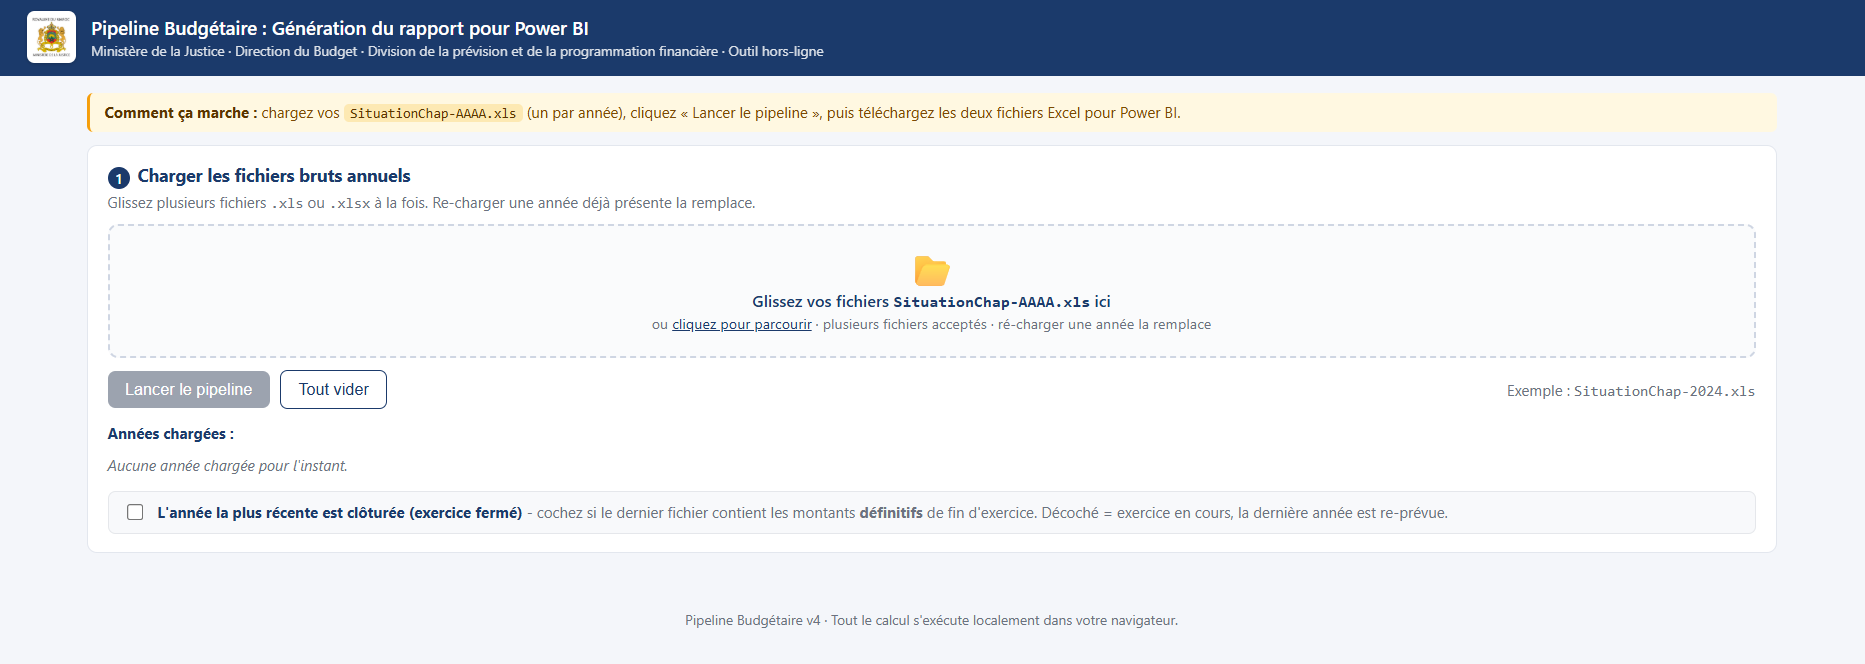
\includegraphics[width=\textwidth]{figures/webapp.png}
    \caption{Interface du fichier HTML autonome livr\'e au gestionnaire. La
    page se compose d'un en-t\^ete identifiant la Direction du Budget et la
    Division de la pr\'evision et de la programmation financi\`ere, d'une
    zone de d\'ep\^ot acceptant le glisser-d\'eposer ou la s\'election des
    fichiers \texttt{SituationChap-AAAA.xls}, et d'une case
    \og exercice cl\^otur\'e \fg{} permettant au gestionnaire de basculer
    entre le mode \emph{exercice en cours} (la derni\`ere ann\'ee est
    re-pr\'evue) et le mode \emph{exercice ferm\'e} (la derni\`ere ann\'ee
    est int\'egr\'ee \`a l'entra\^inement et la pr\'evision triennale d\'ebute
    \`a l'ann\'ee suivante).}
    \label{fig:webapp}
\end{figure}

\begin{itemize}
    \item \emph{T\'el\'echarger \texttt{SituationChap\_RAPPORT\_COMPLET.xlsx}}
    -- contient les feuilles \texttt{R\'ecapitulatif} et \texttt{Donn\'ees}~;
    \item \emph{T\'el\'echarger \texttt{SituationChap\_ANOMALIES.xlsx}}
    -- contient les feuilles \texttt{Anomalies\_Annuelles},
    \texttt{Lignes\_Anormales}, \texttt{Risque\_Combine} et
    \texttt{Decision\_Support}.
\end{itemize}

L'op\'eration peut \^etre r\'ep\'et\'ee autant de fois que n\'ecessaire (par
exemple, apr\`es chaque mise \`a jour mensuelle du fichier de l'exercice en
cours), sans intervention de l'\'equipe informatique.

\subsubsection*{5.3.3 \quad Tra\c{c}abilit\'e et auditabilit\'e}
\addcontentsline{toc}{subsubsection}{5.3.3 \quad Tra\c{c}abilit\'e et auditabilit\'e}

Le code JavaScript de l'outil est int\'egralement lisible (non minifi\'e) et
suffit \`a documenter la cha\^ine de traitement~: chaque coefficient, chaque
seuil, chaque test est inscrit dans le fichier HTML lui-m\^eme, sans
d\'ependance \`a un mod\`ele compil\'e ou pr\'e-entra\^in\'e dont l'auditabilit\'e
serait limit\'ee. Cette propri\'et\'e \og bo\^ite blanche \fg{} est un atout
majeur dans la perspective d'un contr\^ole externe~: le dispositif peut \^etre
int\'egralement reproduit par un tiers \`a partir du seul fichier HTML.

\`A l'ex\'ecution, l'outil restitue \`a l'\'ecran l'ensemble des
informations n\'ecessaires \`a un contr\^ole de premier niveau
(figure~\ref{fig:webapp_results})~: la fen\^etre d'entra\^inement
retenue, le mode \emph{exercice en cours} ou \emph{exercice cl\^otur\'e},
le MAPE m\'edian du \emph{backtest}, le nombre d'anomalies d\'etect\'ees par
chaque m\'ethode et leur r\'epartition par priorit\'e (P0 \`a P4), ainsi
qu'un tableau d\'etaillant pour chaque fichier d\'epos\'e le nombre de
lignes budg\'etaires effectivement extraites. Le gestionnaire dispose
ainsi, avant m\^eme d'ouvrir Power~BI, d'un compte-rendu d'ex\'ecution
qui lui permet de v\'erifier la conformit\'e du traitement et d'identifier
imm\'ediatement tout fichier dont la structure ne correspondrait pas \`a
celle attendue.

\begin{figure}[H]
    \centering
    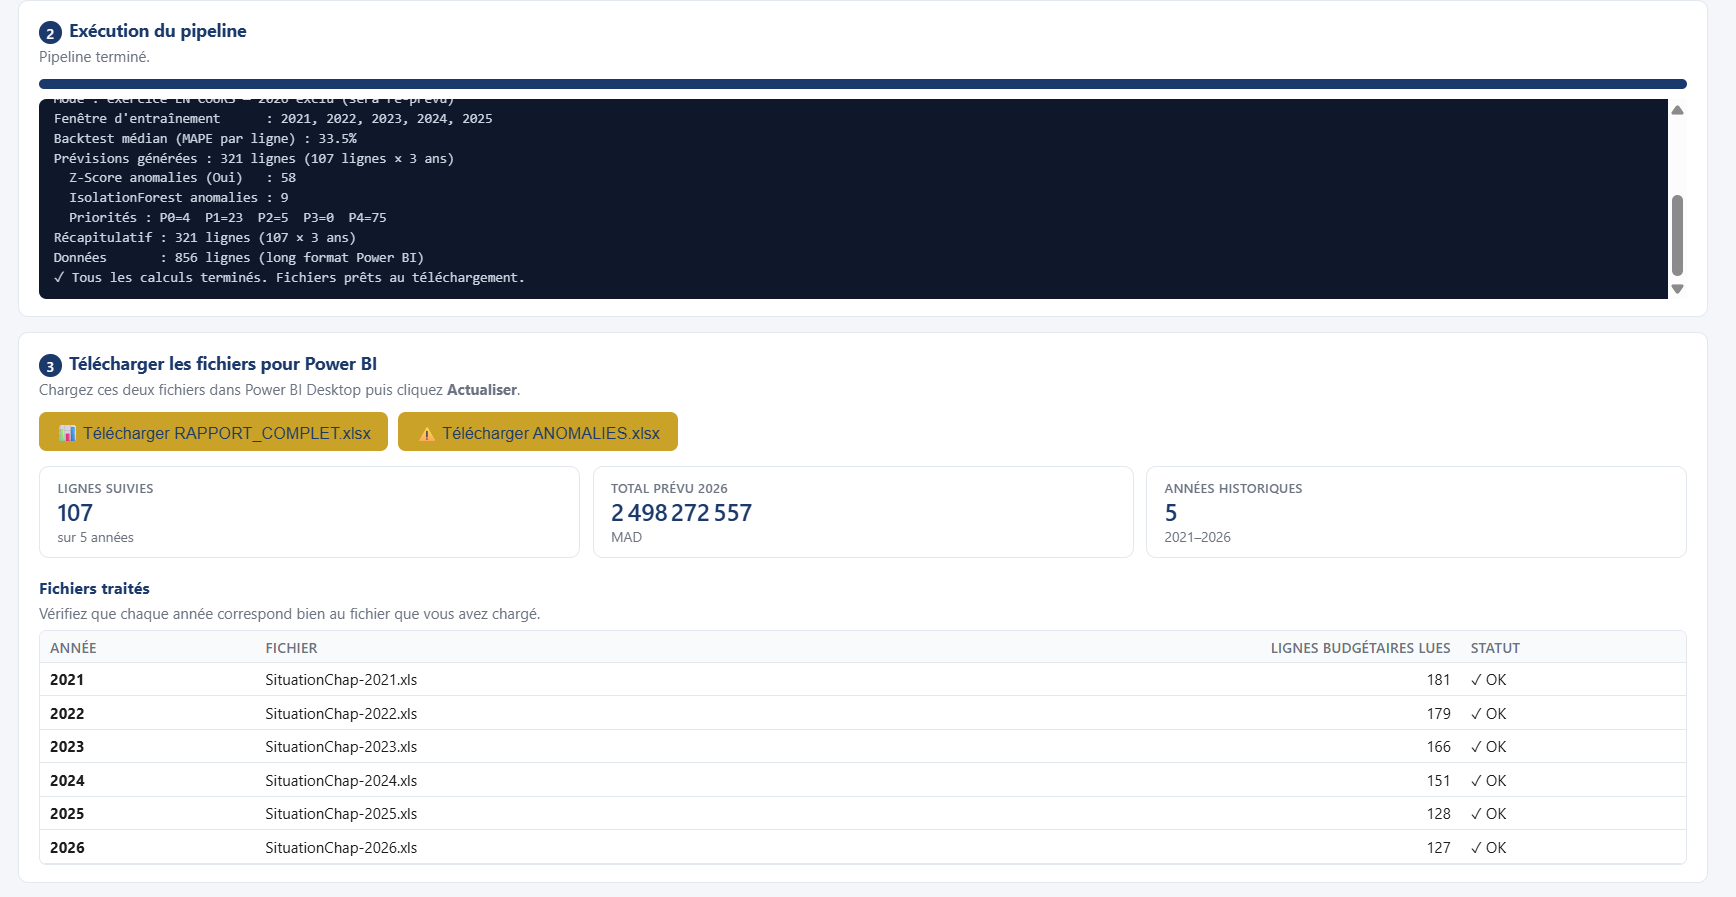
\includegraphics[width=\textwidth]{figures/webapp2.png}
    \caption{Compte-rendu d'ex\'ecution affich\'e par l'outil HTML
    autonome \`a l'issue du traitement. Le journal (haut) trace la
    fen\^etre d'entra\^inement, le MAPE m\'edian par ligne, le nombre
    d'anomalies par m\'ethode et leur r\'epartition par priorit\'e. Les
    indicateurs cl\'es (lignes suivies, total pr\'evu, ann\'ees historiques)
    et le tableau \og fichiers trait\'es \fg{} (un statut par exercice
    avec le nombre de lignes lues) fournissent au gestionnaire une
    auditabilit\'e ligne~\`a~ligne avant export vers Power~BI.}
    \label{fig:webapp_results}
\end{figure}

%================================================================
\phantomsection
\subsection*{5.4 \quad Syst\`eme de pilotage budg\'etaire sous Power BI}
\addcontentsline{toc}{subsection}{5.4 Syst\`eme de pilotage budg\'etaire sous Power BI}
%================================================================

Le second livrable est un fichier \texttt{dashboard.pbix} qui se connecte
aux deux classeurs Excel produits par l'\'etage~1. Power~BI a \'et\'e retenu
parce qu'il est install\'e par d\'efaut sur les postes de la Direction du
Budget, qu'il g\`ere nativement le format \texttt{.xlsx}, et qu'il offre des
filtres crois\'es interactifs sans n\'ecessiter de d\'eveloppement
sp\'ecifique. Le rapport est organis\'e en \textbf{trois pages}, chacune
r\'epondant \`a un usage distinct.

\paragraph{R\^ole du tableau de bord dans le dispositif.}
Le tableau de bord Power~BI ne constitue pas, \`a lui seul, le c\oe ur
d\'ecisionnel du dispositif. Son r\^ole est principalement de restituer
les r\'esultats produits en amont par les modules de pr\'evision et de
d\'etection d'anomalies.

La dimension d'aide \`a la d\'ecision est int\'egr\'ee d\`es la phase de
traitement des donn\'ees. En effet, le syst\`eme ne se limite pas \`a
produire des indicateurs descriptifs~; il g\'en\`ere \'egalement des
niveaux de priorit\'e (P0 \`a P4), des indicateurs de fiabilit\'e, des
alertes d'anomalie et des \'el\'ements d'interpr\'etation destin\'es \`a
orienter l'analyse du gestionnaire.

Ainsi, le dispositif ne cherche pas uniquement \`a r\'epondre \`a la
question \og Que s'est-il pass\'e~?~\fg{}, mais \'egalement \`a identifier
les lignes n\'ecessitant une attention particuli\`ere et \`a hi\'erarchiser
les situations selon leur degr\'e d'urgence. Le tableau de bord constitue
l'interface de consultation de ces r\'esultats, tandis que la logique
d'aide \`a la d\'ecision est port\'ee par les traitements r\'ealis\'es en
amont.

\subsubsection*{5.4.1 \quad Page 1 -- Vue d'ensemble budg\'etaire}
\addcontentsline{toc}{subsubsection}{5.4.1 \quad Page 1 -- Vue d'ensemble budg\'etaire}

La premi\`ere page (figure~\ref{fig:dash-p1}) est destin\'ee \`a la
hi\'erarchie qui cherche un aper\c{c}u synth\'etique. Elle pr\'esente, en
ent\^ete, cinq indicateurs cl\'es~: \emph{Budget Total Ouvert},
\emph{Montant Total Engag\'e}, \emph{Lignes \`a Risque},
\emph{Pr\'ecision Moyenne des Pr\'evisions} et \emph{Taux
d'ex\'ecution moyen}. Quatre visualisations compl\'ementaires
occupent le corps de la page~: l'\'evolution annuelle des cr\'edits ouverts
et de l'engagement r\'eel, la r\'epartition r\'egionale du taux
d'ex\'ecution, le top~5 des \'ecarts au budget, et la moyenne des
engagements par ligne. Trois s\'electeurs (\emph{Ann\'ee},
\emph{Chapitre}, \emph{Ligne Budg\'etaire}) permettent un filtrage
crois\'e instantan\'e.

\begin{figure}[h]
\centering
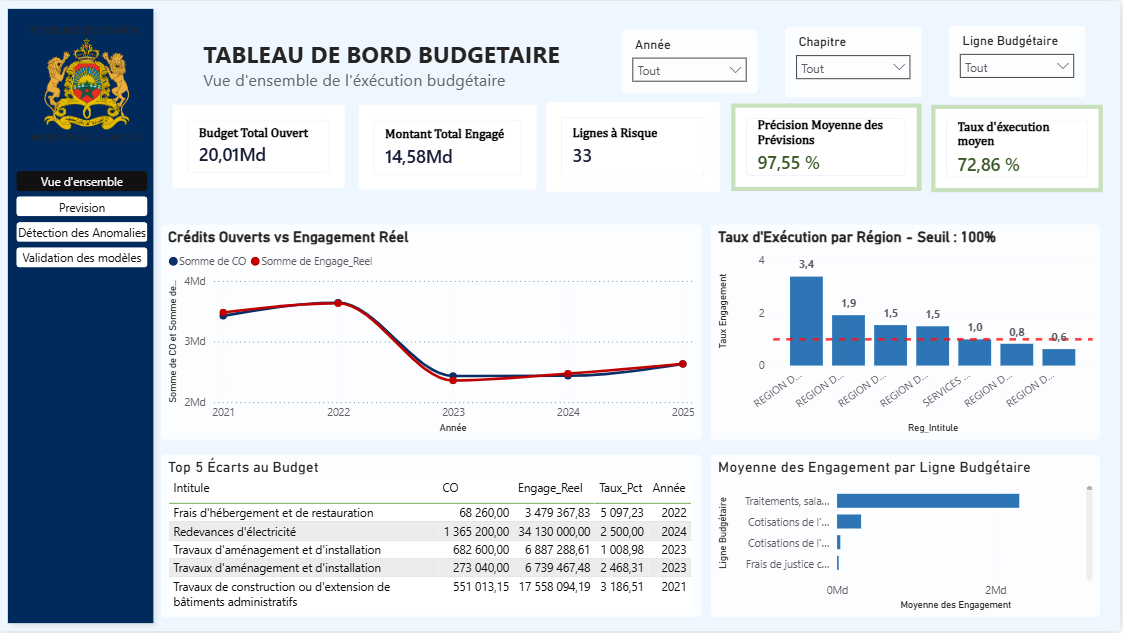
\includegraphics[width=0.95\textwidth]{figures/page1-dash.png}
\caption{Page~1 du tableau de bord Power~BI -- Vue d'ensemble budg\'etaire. KPI agr\'eg\'es en ent\^ete, navigation lat\'erale entre les trois pages, filtres crois\'es Ann\'ee/Chapitre/Ligne.}
\label{fig:dash-p1}
\end{figure}

\subsubsection*{5.4.2 \quad Page 2 -- Suivi des pr\'evisions}
\addcontentsline{toc}{subsubsection}{5.4.2 \quad Page 2 -- Suivi des pr\'evisions}

La deuxi\`eme page (figure~\ref{fig:dash-p2}) est destin\'ee au
contr\^oleur de gestion qui doit instruire la qualit\'e des pr\'evisions
avant leur transmission \`a la Direction du Budget. Elle pr\'esente le
pourcentage de lignes fiables (57{,}94\,\%), le pourcentage de lignes \`a
v\'erifier (39{,}25\,\%), la fiabilit\'e globale (97{,}55\,\%) et le taux
d'erreur global (2{,}45\,\%). Un graphique central confronte la s\'erie des
engagements r\'eels observ\'es \`a la s\'erie pr\'edite par le dispositif sur
l'ensemble du portefeuille, jusqu'\`a l'horizon 2028 inclus. Le tableau
\emph{D\'etail des Pr\'evisions par Ligne Budg\'etaire} permet de descendre
au niveau ligne et de lire, pour chacune, le label Confiance Globale issu
de la section~3.5.2. Un graphique de r\'epartition par Confiance Globale
synth\'etise la distribution des labels (\og Tr\`es fiable \fg{},
\og Fiable \fg{}, \og Acceptable \fg{}, \og Incertain \fg{},
\og \`A v\'erifier \fg{}) sur les 107~lignes.

\begin{figure}[h]
\centering
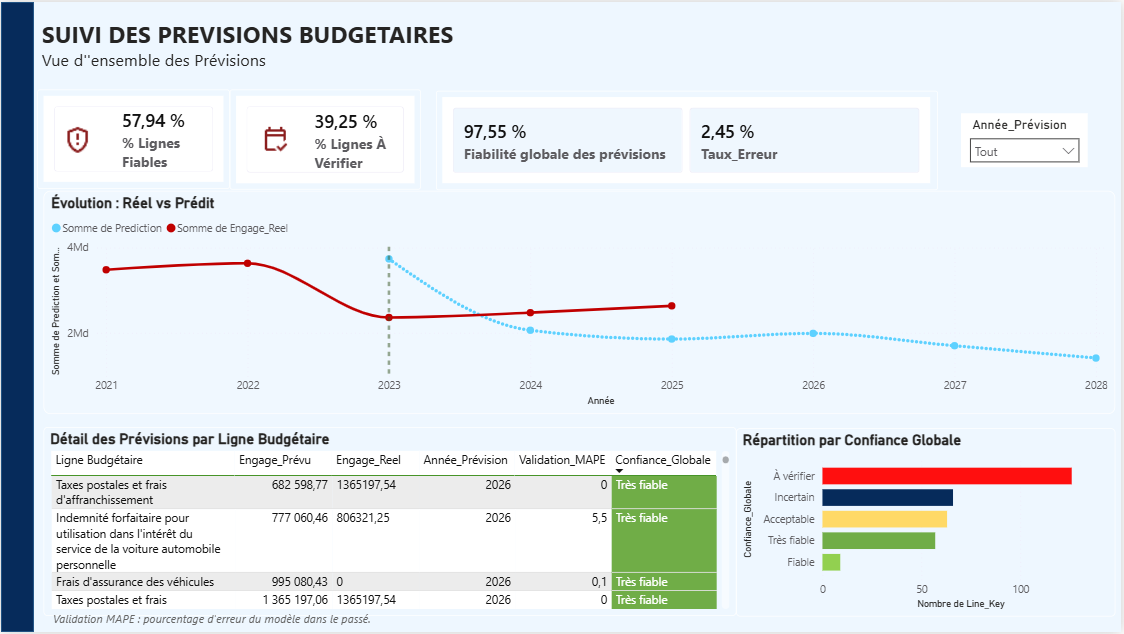
\includegraphics[width=0.95\textwidth]{figures/page2-dash.png}
\caption{Page~2 du tableau de bord Power~BI -- Suivi des pr\'evisions. La ligne pointill\'ee verticale s\'epare les ann\'ees observ\'ees (rouge) des ann\'ees pr\'edites (bleu).}
\label{fig:dash-p2}
\end{figure}

\subsubsection*{5.4.3 \quad Page 3 -- Priorisation des alertes et aide \`a la d\'ecision}
\addcontentsline{toc}{subsubsection}{5.4.3 \quad Page 3 -- Priorisation des alertes et aide \`a la d\'ecision}

La troisi\`eme page (figure~\ref{fig:dash-p3}) est destin\'ee \`a l'usage
op\'erationnel quotidien~: identification des lignes \`a surveiller en
priorit\'e et formulation d'une recommandation d'action. Elle s'ouvre sur
trois indicateurs cl\'es~: la part du portefeuille \`a risque
(32{,}04\,\%), le nombre de lignes critiques (5) et le nombre de lignes
n\'ecessitant une action (27). Le graphique de r\'epartition des lignes
par priorit\'e (Normal, \'Elev\'e, Mod\'er\'e, Critique) refl\`ete
directement la matrice P0--P4 d\'efinie au chapitre~3. Le graphique
central permet d'inspecter la trajectoire du taux d'ex\'ecution d'une ligne
s\'electionn\'ee, et la zone \emph{Explication \& Recommandation} affiche
l'interpr\'etation textuelle issue de la feuille \texttt{Decision\_Support}.
En bas, le tableau \emph{Lignes budg\'etaires prioris\'ees} liste les lignes
class\'ees \og \'Elev\'e \fg{} ou \og Critique \fg{} avec, pour chacune,
l'ann\'ee de derni\`ere anomalie, le taux moyen r\'ecent, une
interpr\'etation et une action recommand\'ee directement actionnable
(\og Renforcer le suivi mensuel \fg{}, \og V\'erifier la cause de l'\'ecart
r\'ecent \fg{}, etc.).

\begin{figure}[h]
\centering
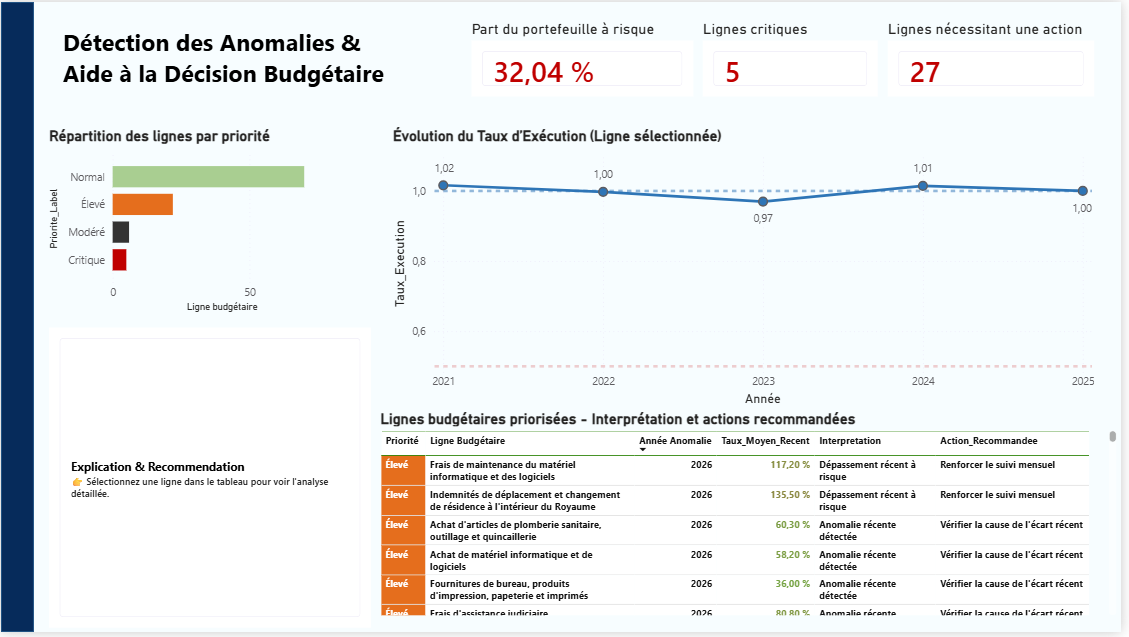
\includegraphics[width=0.95\textwidth]{figures/page3-dash.png}
\caption{Page~3 du tableau de bord Power~BI -- D\'etection des anomalies et aide \`a la d\'ecision budg\'etaire. Le tableau \emph{Lignes budg\'etaires prioris\'ees} traduit chaque alerte en action recommand\'ee.}
\label{fig:dash-p3}
\end{figure}

\subsubsection*{5.4.4 \quad Mod\`ele de donn\'ees Power BI}
\addcontentsline{toc}{subsubsection}{5.4.4 \quad Mod\`ele de donn\'ees Power BI}

Le mod\`ele de donn\'ees du rapport est volontairement minimal~: deux tables
sources (\texttt{R\'ecapitulatif} et \texttt{Donn\'ees}) provenant du
classeur \texttt{RAPPORT\_COMPLET}, deux tables sources
(\texttt{Anomalies\_Annuelles} et \texttt{Decision\_Support}) provenant du
classeur \texttt{ANOMALIES}, et une table calendrier g\'en\'er\'ee par DAX.
Les relations sont \'etablies sur la cl\'e \texttt{Line\_Key} et sur la
colonne \texttt{Ann\'ee}. Cette parcimonie du mod\`ele facilite la
maintenance et garantit qu'un changement de sch\'ema du classeur source
soit imm\'ediatement visible.

%================================================================
\phantomsection
\subsection*{5.5 \quad Apports op\'erationnels}
\addcontentsline{toc}{subsection}{5.5 Apports op\'erationnels}
%================================================================

\subsubsection*{5.5.1 \quad Gain de temps}
\addcontentsline{toc}{subsubsection}{5.5.1 \quad Gain de temps}

Le processus de pr\'evision triennale \og avant outil \fg{} consistait, au
sein du bureau, en une consolidation manuelle des fichiers
\texttt{SituationChap-AAAA.xls}, suivie d'un travail de reconduction
ligne par ligne avec ajustement \og au doigt mouill\'e \fg{}. La dur\'ee
typique de production d'une programmation triennale \'etait de l'ordre de
plusieurs jours-homme. L'outil HTML autonome ram\`ene la production
m\'ecanique \`a moins de cinq secondes~; le gestionnaire concentre alors
son temps sur les 32~lignes prioritaires identifi\'ees par la matrice
P0--P4, l\`a o\`u son expertise apporte de la valeur.

\subsubsection*{5.5.2 \quad Autonomie du gestionnaire}
\addcontentsline{toc}{subsubsection}{5.5.2 \quad Autonomie du gestionnaire}

L'absence de d\'ependance \`a un serveur, \`a un service informatique ou
\`a une plateforme cloud signifie que le gestionnaire peut~: (i) ex\'ecuter
l'outil hors ligne~; (ii) le partager par simple copie du fichier \`a un
coll\`egue~; (iii) le faire \'evoluer en demandant une modification au
prestataire sans n\'ecessiter de cycle de validation DSI~; (iv) le verser
\`a une archive p\'erenne (le fichier reste fonctionnel ind\'efiniment).

\subsubsection*{5.5.3 \quad Tra\c{c}abilit\'e et redevabilit\'e}
\addcontentsline{toc}{subsubsection}{5.5.3 \quad Tra\c{c}abilit\'e et redevabilit\'e}

Chaque chiffre publi\'e par le dispositif est accompagn\'e du nom du
mod\`ele s\'electionn\'e (colonne \texttt{Mod\`ele\_Utilis\'e}), du MAPE de
validation (colonne \texttt{Validation\_MAPE}) et du label Confiance
Globale. Cette tra\c{c}abilit\'e satisfait l'exigence de redevabilit\'e
identifi\'ee au chapitre~3~: aucune
pr\'evision n'est livr\'ee sans son \og pedigree \fg{} statistique, et
toute critique externe peut \^etre instruite ligne par ligne.

\subsubsection*{5.5.4 \quad Articulation avec les processus existants}
\addcontentsline{toc}{subsubsection}{5.5.4 \quad Articulation avec les processus existants}

Le double livrable s'ins\`ere dans le calendrier budg\'etaire sans le
bouleverser. L'outil HTML est destin\'e \`a \^etre relanc\'e \`a trois
moments cl\'es de l'ann\'ee~: en \textbf{mars-avril}, lors de la
pr\'eparation des arbitrages pour le PLF $N+1$~; en \textbf{septembre}, lors
du bouclage du PLF d\'epos\'e au Parlement~; en \textbf{janvier}, apr\`es
publication de la loi de finances vot\'ee, pour mettre \`a jour le tableau
de bord Power~BI avec les cr\'edits ouverts d\'efinitifs. Le tableau de
bord est consult\'e en continu par la Direction du Budget pour suivre
l'ex\'ecution de l'exercice en cours.

%================================================================
\phantomsection
\subsection*{5.6 \quad Limites et perspectives}
\addcontentsline{toc}{subsection}{5.6 Limites et perspectives}
%================================================================

\subsubsection*{5.6.1 \quad Limites du livrable actuel}
\addcontentsline{toc}{subsubsection}{5.6.1 \quad Limites du livrable actuel}

Quatre limites doivent \^etre reconnues~:

\textbf{Premi\`erement}, l'outil HTML traite des donn\'ees annuelles~: il
n'exploite pas l'information infra-annuelle (engagements mensuels,
ordonnancements trimestriels) qui pourrait pourtant am\'eliorer la
d\'etection pr\'ecoce des d\'erives. L'int\'egration des donn\'ees
mensuelles issues du GID, lorsque celles-ci seront accessibles dans un
format standardis\'e, constitue la principale piste d'enrichissement.

\textbf{Deuxi\`emement}, le tableau de bord Power~BI suppose que les
fichiers \texttt{.xlsx} sources soient stock\'es \`a un emplacement
accessible par tous les utilisateurs (typiquement, un partage r\'eseau du
bureau). Une migration vers un d\'ep\^ot interne s\'ecuris\'e (SharePoint
on-premise, par exemple) faciliterait le partage multi-utilisateur sans
remettre en cause les contraintes de s\'ecurit\'e.

\textbf{Troisi\`emement}, l'outil ne propose pas de m\'ecanisme natif de
versionnement des productions~: deux ex\'ecutions successives produiront
deux classeurs portant le m\^eme nom, dont la diff\'erence ne sera
trac\'ee que par la date de fichier. Une \'evolution simple consisterait
\`a horodater automatiquement les fichiers de sortie.

\textbf{Quatri\`emement}, la \textit{robustesse vis-\`a-vis de
l'\'evolution des fichiers sources}. Le fonctionnement du dispositif
repose sur la structure actuelle des fichiers \texttt{SituationChap-AAAA.xls}
produits par le syst\`eme d'information budg\'etaire. Une modification
significative du format des fichiers sources (renommage des colonnes,
ajout ou suppression de champs, changement de structure) pourrait
n\'ecessiter une adaptation du module d'importation. Cette d\'ependance
constitue une limite classique des syst\`emes de traitement automatis\'e
de donn\'ees. Dans une perspective de d\'eploiement \`a long terme, une
\'evolution du dispositif pourrait int\'egrer des m\'ecanismes de
validation du sch\'ema d'entr\'ee ainsi que des contr\^oles de coh\'erence
permettant de d\'etecter automatiquement les changements de structure
avant le lancement des traitements.

\subsubsection*{5.6.2 \quad Perspectives d'\'evolution}
\addcontentsline{toc}{subsubsection}{5.6.2 \quad Perspectives d'\'evolution}

Quatre directions d'\'evolution sont envisageables, par ordre croissant
d'investissement~:

\begin{enumerate}
    \item \textbf{Enrichissement de la matrice de priorit\'e} par
    int\'egration de seuils manuels (\og lignes politiquement sensibles \fg{},
    \og lignes en restructuration \fg{}) qui forceraient un classement
    minimal ind\'ependamment du score statistique.
    \item \textbf{Module de simulation \og what-if \fg{}}~: permettre au
    gestionnaire de modifier interactivement un cr\'edit ouvert ou un
    taux d'ex\'ecution cible, et d'observer l'impact sur les pr\'evisions
    et sur les anomalies.
    \item \textbf{Bascule vers les donn\'ees mensuelles GID} d\`es qu'un
    flux automatis\'e sera disponible, avec un mod\`ele saisonnier
    appropri\'e (lissage exponentiel de Holt-Winters, par exemple, sous
    r\'eserve d'une profondeur historique suffisante).
    \item \textbf{Extension du dispositif \`a d'autres minist\`eres}~:
    l'architecture en pipeline et l'ind\'ependance vis-\`a-vis du contenu
    sp\'ecifique du Minist\`ere de la Justice permettent une transposition
    rapide \`a tout d\'epartement minist\'eriel utilisant la nomenclature
    LOF~130-13.
\end{enumerate}

%================================================================
\phantomsection
\subsection*{5.7 \quad Synth\`ese du chapitre}
\addcontentsline{toc}{subsection}{5.7 Synth\`ese du chapitre}
%================================================================

Ce chapitre a montr\'e comment un dispositif statistique th\'eoriquement
solide -- valid\'e empiriquement au chapitre~4 -- peut \^etre transform\'e
en un outil concr\`etement utilisable dans un environnement institutionnel
exigeant. Trois principes ont guid\'e l'architecture~:

\begin{itemize}
    \item \textbf{Conformit\'e aux contraintes r\'eelles}~: aucun choix
    technique n'a \'et\'e fait sans int\'egrer les contraintes de
    s\'ecurit\'e informatique du minist\`ere -- d'o\`u le rejet d'une
    application compil\'ee au profit d'un fichier HTML autonome.
    \item \textbf{S\'eparation des responsabilit\'es}~: l'\'etage de
    production et l'\'etage de pilotage sont d\'ecorr\'el\'es par une
    interface explicite (les classeurs Excel), ce qui autorise des
    \'evolutions ind\'ependantes.
    \item \textbf{Autonomie du gestionnaire}~: l'outil est con\c{c}u pour
    ne d\'ependre ni d'un service informatique central, ni d'une
    connexion r\'eseau, ni d'un prestataire externe pour son ex\'ecution.
\end{itemize}

Le double livrable r\'epond ainsi \`a l'engagement m\'ethodologique pos\'e
en introduction~: faire de la parcimonie statistique non un repli par
d\'efaut, mais une exigence positive qui irrigue \emph{aussi} les choix
d'ing\'enierie. La \textbf{Conclusion g\'en\'erale} revient sur l'ensemble
du parcours et discute les enseignements transverses du travail.
